\documentclass[11pt, a4paper]{scrreprt} % fontsize, format, art des dokuments

\usepackage[utf8]{inputenc} % ermoeglicht Verwendung von Unicode
\usepackage{graphicx} % zum einfuegen von grafiken
  \graphicspath{ {figures/} } % gibt an wo die Grafiken sind
\usepackage[german]{babel} % zum umstellen auf deutsch
\usepackage{csquotes} % wegen babel, zum zitieren mit "" sonst warnung
\newcounter{savepage} % Zähler zum weiterzählen der römischen Zahlen
\usepackage[hidelinks]{hyperref}
\usepackage{float}
\usepackage{booktabs}
\usepackage{tabularx} % zum leichteren nutzen von tabellen
\setlength{\parindent}{0em} % indent wegmachen
\usepackage{listings}
\usepackage[linesnumbered,ruled,vlined]{algorithm2e}
\usepackage{algorithmic}
\usepackage{amsmath}
\usepackage{float}
\usepackage[acronym]{glossaries}
\usepackage{subcaption} % praktisch, wenn man eine Grafik aus zwei Grafiken oder mehr macht

%Setting counters for citations, tables and figures
\AtBeginDocument{\counterwithin{lstlisting}{section}%
             \renewcommand\thelstlisting{\arabic{lstlisting}}}
\usepackage[style=numeric, backend=biber, sorting = none]{biblatex} % gute Moeglichkeit seine Quellen zu verwalten
  \addbibresource{bibliography/resources.bib} % In dieser Datei liegen dann die Quellen
\counterwithout{figure}{chapter} % Figures werden absolut gezaehlt und nicht nach Kapitel
\counterwithout{table}{chapter} % Tables werden absolut gezaehlt und nicht nach Kapitel



\makeglossaries

\newacronym{COVID 19}{COVID 19}{coronavirus disease 2019}

\newacronym{SARS-CoV-2}{SARS-CoV-2}{severe acute respiratory syndrome coronavirus type 2}

\newacronym{plDDT}{plDDT}{predicted local distance difference test}

\newacronym{CASP}{CASP}{Critical Assessment of Protein Structure Prediction}

\newacronym{GPU}{GPU}{graphics processing unit}

\newacronym{AI}{AI}{artificial intelligence} 

\newacronym{RMSD}{RMSD}{root-mean-square deviation} 

\newacronym{Cameo3D}{Cameo3D}{Continuous Automated Model EvaluatiOn} 

\newacronym{Phyre2}{Phyre2}{Protein Homology/analogY Recognition Engine V 2.0} 

\newacronym{RNP}{RNP}{ribonucleocapsid}

\newacronym{RNA}{RNA}{ribonucleic acid}

\newacronym{DNA}{DNA}{deoxyribonucleic acid} 

\newacronym{NSP}{NSP}{Non-structural protein} 

\newacronym{ACE2}{ACE2}{angiotensin-converting enzyme 2} 

\newacronym{BFD}{BFD}{Big Fantastic Database} 

\newacronym{MSA}{MSA}{Multiple Sequence Alignment} 

\newacronym{HMM}{HMM}{Hidden Markov Model} 

\newacronym{ENA}{ENA}{European Nucleotide Archive} 

\newacronym{PDB}{PDB}{Protein Data Bank} 

\newacronym{PSI-BLAST}{PSI-BLAST}{Position-Specific Iterative Basic Local Alignment Search Tool}

\newacronym{VRAM}{VRAM}{video random access memory} 

\newacronym{RAM}{RAM}{random access memory} 

\newacronym{HDD}{HDD}{hard disk drive} 

\newacronym{NVMe}{NVMe}{nonvolatile memory express} 

\newacronym{SSD}{SSD}{solid state drive} 

\newacronym{lDDT-C}{lDDT-C}{local distance difference test-C}

\newacronym{mmCIF}{mmCIF}{macro-molecular Crystallographic Information File} 

\newacronym{PNG}{PNG}{portable network graphic} 

\newacronym{URL}{URL}{uniform resource locator} 

\newacronym{iCn3D}{iCn3D}{I see in 3D} 


\begin{document}

	\pagenumbering{Roman}
	\begin{titlepage}

	\begin{figure}
	
\includegraphics[width=1\textwidth]{th_bingen.png}
	\end{figure}
	
	\begin{center}
	\large
	TH Bingen Technical University of Applied Sciences\\
    Department 2 - Technology, Informatics and Economics\\
    Applied Bioinformatics (B.Sc.)\\
    \vspace{0.5cm}
	
    \huge
    \textbf{Gene Expression Analyses on yeast heat
shock experiments} 
    \vfill
    
    \large
    Prüfungsleistung: Data Mining with R \\
    Abgegeben am: 11.02.2025 \\
    Name: Robin Ender \\
    Matrikelnummer: 2184737
    \vspace{0.5cm}
	\end{center}
	
\end{titlepage}


	The Abstract is a short summary of the scientific publication that usually
contains a short description of the publications topic to help the reader to
decide whether to read the full paper or not. Optimally the reader is convinced
to read the full paper after the author generated enough interest. The Abstract
prepares the readers for the detailed an in-depth processes of the topic. At
last, an abstract helps the reader to remember key points from the publication.
Citations must be done in this style:

	\listoffigures
	\listoftables
	\tableofcontents
	\cleardoublepage
	
	\setcounter{savepage}{\arabic{page}} 
	\pagenumbering{arabic}
	\chapter{Introduction}

\section{questions to answer}
The Introduction mostly answers the following questions in a short manner:
\begin{itemize}
	\item What is the topic of this scientific publication?
	\item What is the current point of research?
	\item What materials and which methods were used to work on the topic?
	\item What is the hypothesis, that was to confirm or deny?
    \item This is an example for a citation (\cite{Beispiel1}). % Siehe dazu auch ./bibliography/resources.bib

\end{itemize}

\section{Introduction style}
An Introduction is written in plain text, and is usually written as one
paragraph of continuing text, although it is also possible to subdivide the
text into different partitions.

\subsection{This is a sub-section}

Lorem ipsum bla foo bar...

  \chapter{Material}

As described in the introduction, we used existing data from a heat shock experiment. 
The origin of this data as well as of the reference data is shown in 
table~\ref{tab:Material}.

\begin{table}[H]
  \center
  \caption{Data used in this work.}\label{tab:Material}
  \begin{tabular}{llll}
    \toprule
    
    Description & Database & Identifier & Version or Date created \\
    \midrule
    RNA-seq data & NCBI GEO & GSE135568 &  Mar 09, 2020\\
    Reference genome & SGD & S288C & version=R64-4-1 2024-05-29 \\ 
    Gene Ontology & UniProt & GO & 2024-12-15 \\
    \bottomrule
  \end{tabular}
\end{table}

% accesion date neccesary? 

	\chapter{Methods}
\section{Reproduction}
Throughout the whole paper there is a need to describe every detail and every
step in a precise manner to make sure all created results can be reproduced by
others. First and foremost this reproduction demand has to be ensured in the
"methods" chapter.

Also very important are:
\begin{itemize}
	\item A chronological order of all steps (including software versions,
	details, data-handling, ..) 
	\item What method was used to solve each part of the task?  
	\item What data versions created which results?
\end{itemize}

\begin{figure}[ht]
    \centering
    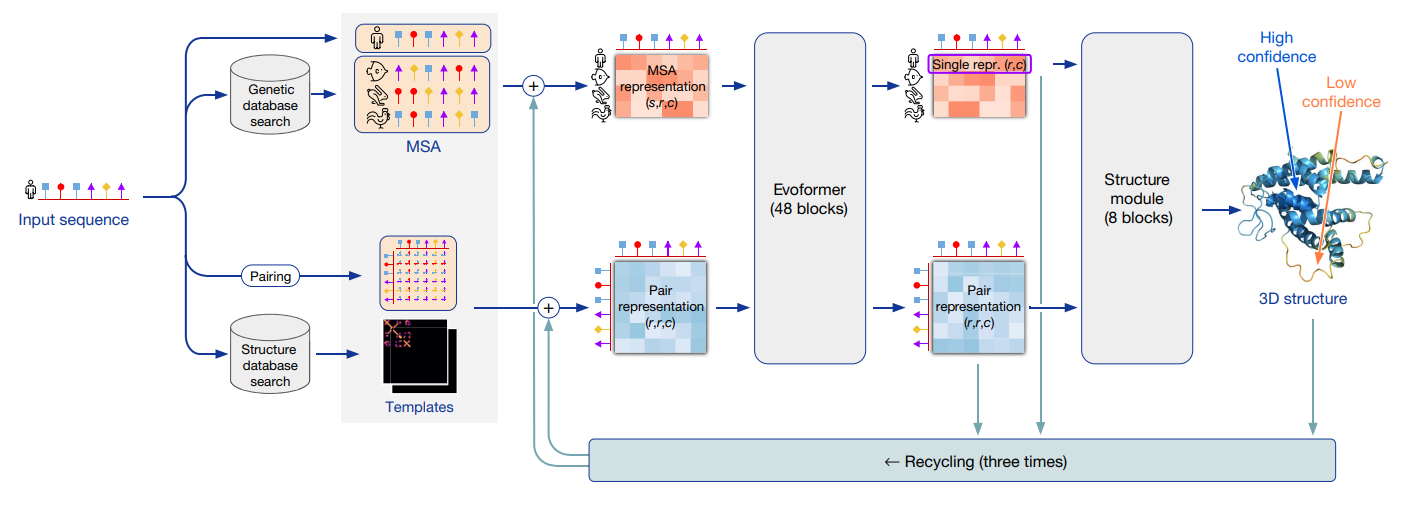
\includegraphics[width=1\textwidth]{figures/alphafold_architecture.png}
    \caption{Example of a captiones figure}
    \label{modelarch}
\end{figure}
This is a single-line code example:
\begin{verbatim}
    $ docker run --rm --gpus all nvidia/cuda:11.0-base nvidia-smi
\end{verbatim}
\section{Formula examples}
Scores below 0.2 belong to randomly selected unrelated proteins, according 
to stringent statistics of structures in the \acrshort{PDB}, while those with
more than 0.5 generally have the same protein fold (\cite{Beispiel1}) oder \parencite{Beispiel1}. The TM-score
is calculated defined by:
\[ TM-score = max 
\begin{bmatrix}
\label{complex_formula_1}
\frac{1}{L_{target}}\sum_{i}^{L_{common}} \frac{1}{1+(\frac{d_i}{d_0(L_{target})})^2}
\end{bmatrix}\]
Where L$_{target}$ is the length of the amino acid sequence of the target
protein, and L$_{common}$ is the number of residues that appear in both the
template and target structures, d$_{i}$ is the distance between the $i$th pair
of residues in the template and target structures, and $d_{0} (L_{target})$ is
a distance scale that normalizes distances and is defined by:
\[ d_{0} (L_{target}) = 1.24\sqrt[3]{L_{target}-15-1.8} \]

This is a refererence to the labeled (numbered) formula [\ref{complex_formula_1}]
When comparing two protein structures that have the same residue order, L$_{common}$ 
reads from the C-alpha order number of the structure files. The \acrshort{RMSD}
value is defined by: \[ RMSD = \sqrt{\frac{1}{N}\sum_{i=1}^{N} \delta i^2} \]
Where $\delta$i is the distance between atom i and either a reference structure 
or the mean position of the N equivalent atoms.


\begin{table}[H]
  \begin{center}
    \caption[Distribution of values tested during simulated annealing in 4th
    quartile of high scoring parameter sets]{Distribution of values tested during
    simulated annealing in 4th quartile of high scoring parameter sets (mean
    F2-Scores $>$ 0.6454).}
    \begin{tabular}{c r r r r r r r}%
      \toprule{}%
      Parameter & Minimum & 1st Quartile & Median & Mean \\
      \midrule{}%
      $\alpha$        & 0.1000 & 0.2000 & 0.4000 & 0.4692     \\
      $\beta$         & 0.0476 & 0.3704 & 0.4545 & 0.4622     \\
      $\omega$        & 0.0476 & 0.1250 & 0.2105 & 0.2324     \\
      $\sigma$        & 0.0476 & 0.1875 & 0.3077 & 0.3054     \\
      Sprot-$w$       & 10.0000 & 20.0000 & 30.0000 & 41.02009738 \\
      Sprot-$\delta$  & 0.1000 & 0.3000 & 0.5000 & 0.5365    \\
      trEMBL-$w$      & 10.0000 & 50.0000 & 70.0000 & 67.10005704 \\
      trEMBL-$\delta$ & 0.1000 & 0.5000 & 0.7000 & 0.6823     \\
      TAIR-$w$        & 10.0000 & 30.0000 & 50.0000 & 53.79005853 \\
      TAIR-$\delta$   & 0.1000 & 0.3000 & 0.5000 & 0.5392     \\
      \bottomrule{}%
    \end{tabular}
    \label{tbl:value_table}
  \end{center}
\end{table}

This is an example on how to reference a table that has the
\verb|\label{tbl:value_table}| by using \verb|\ref{tbl:value_table}|: The
estimated values are listed in table \ref{tbl:value_table}.

	\chapter{Results}

\section{Envelope Variants}

\begin{figure}[H]
\centering
	\begin{subfigure}[b]{0.45\textwidth}
		\centering
		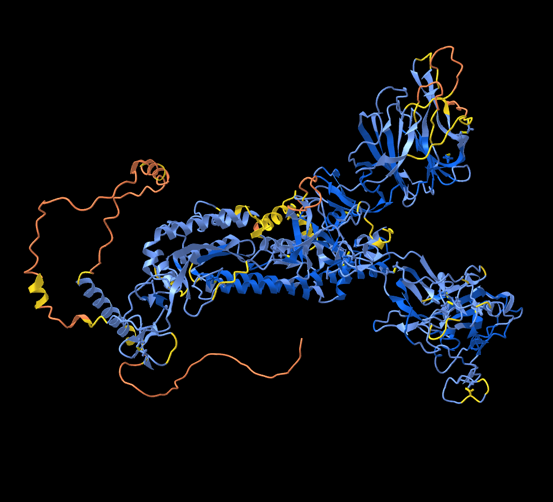
\includegraphics[width=\textwidth]{figures/gu280_ref.png}
		\caption{Left part of a figure partitioned into subfigures.}
		\label{plddtCon2a}
	\end{subfigure}
	\hfill
	\begin{subfigure}[b]{0.49\textwidth}
		\centering
		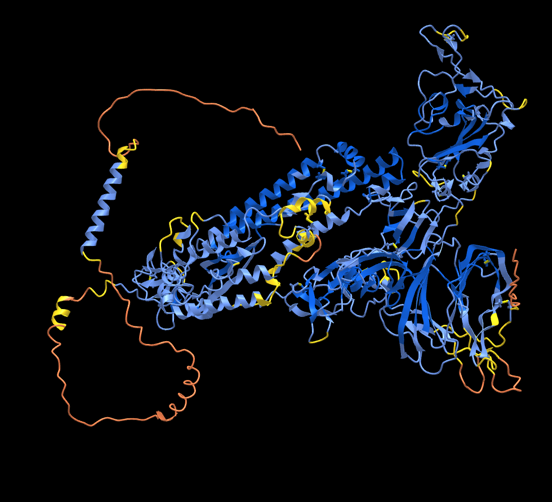
\includegraphics[width=\textwidth]{figures/gu280_var3.png}
		\caption{Right part of a figure partitioned into subfigures.}
		\label{plddtCon2b}
	\end{subfigure}
	\caption{An example of a subdivided figure.}
	\label{subfigure_this}
\end{figure}

As we have labeled the above figure containing subfigures, we can reference it using \ref{subfigure_this}.

\begin{figure}[H]
	\centering
	\fbox{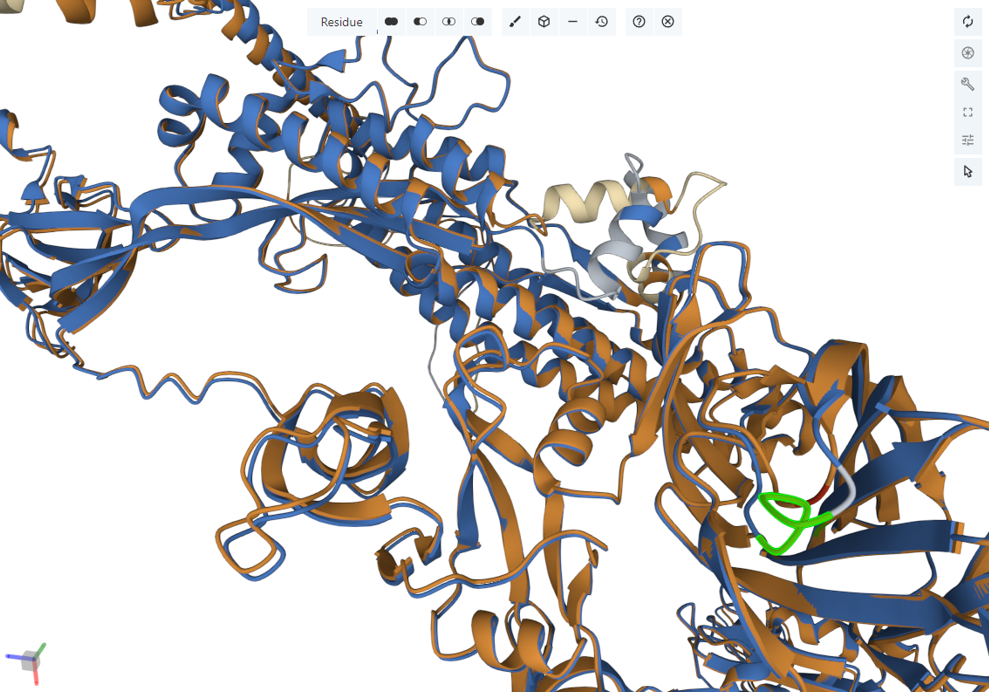
\includegraphics[width=0.9\textwidth]{figures/gu280_var3_comp_close.png}}
	\caption{An example of an unsubdivided figure.}
	\label{figured_out}
\end{figure}

Similarly, we can reference the unsubdivided figure using \ref{figured_out}.

\section{Code Example}

The results of the study include the generated data, outcomes of statistical tests, and visual evaluations such as plant leaf imagery. This section focuses on presenting these results objectively without interpretation. Incremental values can be depicted using tables and figures where necessary.

Below is an example of how to insert an algorithm in LaTeX:

\begin{algorithm}[H]

\KwData{
\begin{itemize}
    \item $g$: The GO term to compute the mutation probability lookup table for.
    \item $\mathcal{H}$: The \emph{ordered} set of homologous protein pairs $p_i$, where\\
    \hspace{1cm} at least one member has annotation $g$,\\
    \hspace{1cm} with $\mathcal{G}_x$ as the set of GO term annotations of protein $x$: \\
    \hspace{1cm} $p_i = \{ \, p_i^1, p_i^2 ~ | ~ \exists ~ k \in \{1,2\} : g \in \mathcal{G}_{p_i^k} \, \}$, and\\
    \hspace{1cm} each pair $p_i$ has a sequence distance $d_i$ such that: $d_{i-1} \leq d_i$.
\end{itemize}
}
\KwResult{
\begin{itemize}
    \item $M$: Ordered set of mutation probabilities $P( \, g^{mut} \,|\, d_k \,)$, with\\
    \hspace{1cm} $m_{k-1} \leq m_k$ for $d_{k-1} \leq d_k$.
\end{itemize}
}

\BlankLine
\textbf{Initialize:}\\
$n_{not\_sharing} \leftarrow 0$\\
$n_{all} \leftarrow 0$\\
$m_{candidate} \leftarrow 0$\\
$m_{current} \leftarrow 0$\\
\BlankLine

\ForEach{$p_i \in \mathcal{H}$, $1 \leq i \leq |\mathcal{H}|$}{
    Increment $n_{all}$ by 1.\\
    \If{$\exists ~ k \in \{1,2\} : g \notin \mathcal{G}_{p_i^k}$}{
        Increment $n_{not\_sharing}$ by 1.\\
    }
    $m_{candidate} \leftarrow \frac{n_{not\_sharing}}{n_{all}}$\\
    \If{$m_{candidate} > m_{current}$}{
        $m_{current} \leftarrow m_{candidate}$\\
        Append $m_{current}$ to $M$.\\
    }
}
\caption{Mutation Probability Lookup Algorithm}
\label{alg:mutation_lookup}
\end{algorithm}


\section{Example of using a reference to another section}

This is a reference example. To reference the code example above, simply use \\
\verb|\ref{alg:mutation_lookup}| \ref{alg:mutation_lookup}.

Find more information about the materials in section \ref{Topics_of_Material} \\
(\verb|\ref{Topics_of_Material}|) on page \pageref{Topics_of_Material}
(\verb|\pageref{Topics_of_Material}|).

	\chapter{Discussion}

	\cleardoublepage
	
	\pagenumbering{Roman}
	\setcounter{page}{\thesavepage}
	\printbibliography
	
	\cleardoublepage
	\pagenumbering{gobble}
	\leavevmode
\vfill

\begin{center}
\textbf{Erklärung zur Originalität der Arbeit}
\end{center}
Hiermit bestätige ich, dass die abgegebene Arbeit das Original ist und von mir ohne weitere Hilfe geschrieben wurde. Wenn Arbeit anderer referenziert oder genutzt wurde, wurde dies angemessen kenntlich gemacht. Meine Arbeit wurde noch nicht bewertet oder veröffentlicht. Die elektronisch abgegebene Version stimmt mit der elektronischen überein.

\vspace{1cm}
\hfill
\begin{tabular}[t]{c}
  \rule{10em}{0.4pt}\\ Unterschrift
\end{tabular}
\hfill
\begin{tabular}[t]{c}
  \rule{10em}{0.4pt}\\ Ort und Datum
\end{tabular}
\hfill
\strut
\vspace{2cm}


\begin{center}
\textbf{Erklärung zum Eigentum und Urheberrecht}
\end{center}
Hiermit erkläre ich meine Zustimmung, dass die Technische Hochschule Bingen diede Arbeit anderen Studierenden und interessierten Dritten zur Verfügung stellen und in meinem Namen (Robin Ender) veröffentlichen darf.

\vspace{1cm}
\hfill
\begin{tabular}[t]{c}
  \rule{10em}{0.4pt}\\ Unterschrift
\end{tabular}
\hfill
\begin{tabular}[t]{c}
  \rule{10em}{0.4pt}\\ Ort und Datum
\end{tabular}
\hfill
\strut
\vfill


	
\end{document}
